%!TEX TS-program = xelatex
\documentclass[]{friggeri-cv}
\usepackage{afterpage}
\usepackage{hyperref}
\usepackage{color}
\usepackage{xcolor}
\usepackage{smartdiagram}
\usepackage{fontspec}
% if you want to add fontawesome package
% you need to compile the tex file with LuaLaTeX
% References:
%   http://texdoc.net/texmf-dist/doc/latex/fontawesome/fontawesome.pdf
%   https://www.ctan.org/tex-archive/fonts/fontawesome?lang=en
%\usepackage{fontawesome}
\usepackage{metalogo}
\usepackage{dtklogos}
\usepackage[utf8]{inputenc}
\usepackage{tikz}
\usetikzlibrary{mindmap,shadows}
\hypersetup{
    pdftitle={},
    pdfauthor={},
    pdfsubject={},
    pdfkeywords={},
    colorlinks=false,           % no lik border color
    allbordercolors=white       % white border color for all
}
\smartdiagramset{
    bubble center node font = \footnotesize,
    bubble node font = \footnotesize,
    % specifies the minimum size of the bubble center node
    bubble center node size = 0.5cm,
    %  specifies the minimum size of the bubbles
    bubble node size = 0.5cm,
    % specifies which is the distance among the bubble center node and the other bubbles
    distance center/other bubbles = 0.3cm,
    % sets the distance from the text to the border of the bubble center node
    distance text center bubble = 0.5cm,
    % set center bubble color
    bubble center node color = pblue,
    % define the list of colors usable in the diagram
    set color list = {lightgray, materialcyan, orange, green, materialorange, materialteal, materialamber, materialindigo, materialgreen, materiallime},
    % sets the opacity at which the bubbles are shown
    bubble fill opacity = 0.6,
    % sets the opacity at which the bubble text is shown
    bubble text opacity = 0.5,
}

\addbibresource{bibliography.bib}
\RequirePackage{xcolor}
\definecolor{pblue}{HTML}{0395DE}

\begin{document}
\header{Long }{Nguyen}
      {Computer Engineer}
      
% Fake text to add separator      
\fcolorbox{white}{gray}{\parbox{\dimexpr\textwidth-2\fboxsep-2\fboxrule}{%
.....
}}


% In the aside, each new line forces a line break
\begin{aside}
%scale 0.35 for long.JPG
  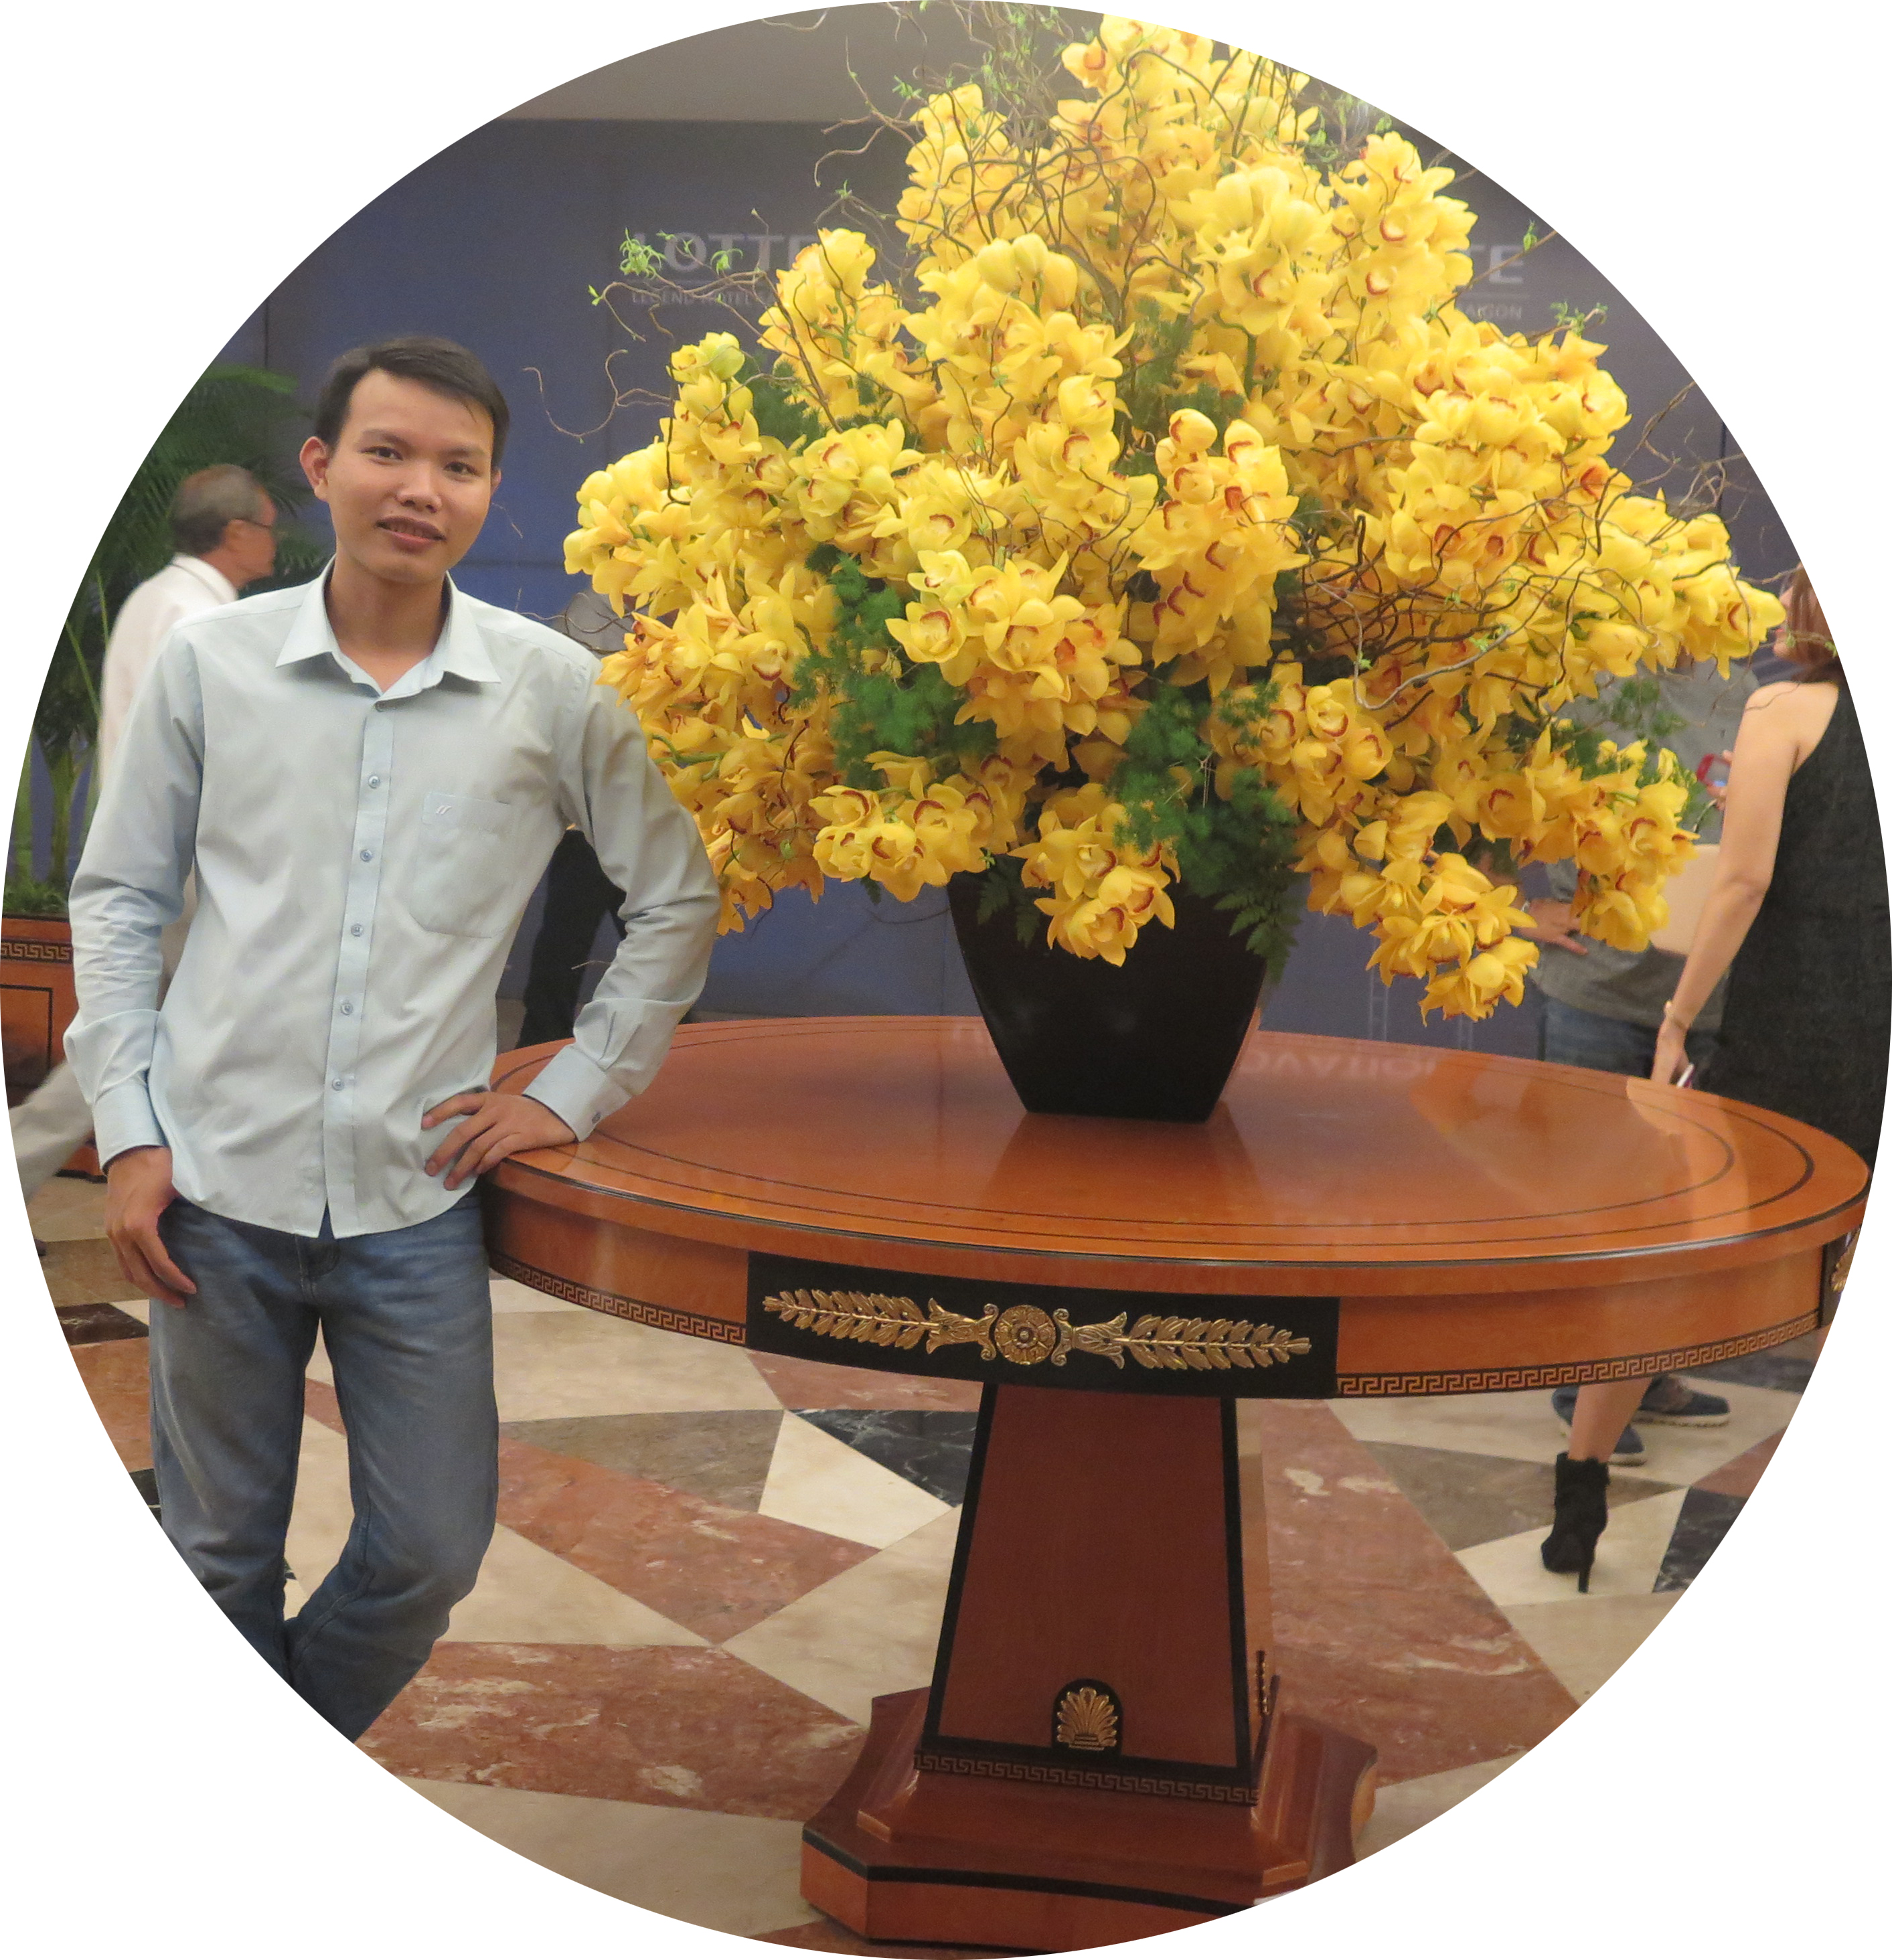
\includegraphics[scale=0.1]{img/kalog-noedit.jpg}
  \section{Full Name}
Nguyen Quoc Long
  \section{Gender}
Men
  \section{Date of birth}
    %\href{mailto:longnguyencse@gmail.com}{\textbf{longnguyencse@}\\gmail.com}
05/1993
~
~
~
~
 % \section{Web \& Git}
    %\href{http://mywebsite.com}{https://longbkitblog
	%.wordpress.com/}
    %\href{https://bitbucket.org/mygit}{bitbucket.org/mygit}
  %  \href{https://github.com/mygit}{https://github.com
	%/longnguyencse}
    %\href{https://gitlab.com/u/mygit}{gitlab.com/u/mygit}
    %~
  % use  \hspace{} or \vspace{} to change bubble size, if needed
  \section{Programming}
    \smartdiagram[bubble diagram]{
        \textbf{Java},
        \textbf{Python},
        \textbf{C/C++},
%        \textbf{Lua/UCI},
        \textbf{Other\vspace{3mm}},
        \textbf{HTML/CSS}\\\textbf{JS/jQuery},
        \textbf{PHP},
   %    \textbf{Android},
        \textbf{Bash}
    }
    ~
  \section{Personal Skills}
~
    \smartdiagram[bubble diagram]{
        \textbf{Team}\\\textbf{Player},
      %  \textbf{Initiative}, % sang kien
        \textbf{Curiosity}, % ham hieu biet
        \textbf{Problem}\\\textbf{Solving},
        \textbf{\vspace{1mm}Manage\vspace{1mm}},
        \textbf{Organize}
    }
    ~
\end{aside}
~

\section{Person Information}
\begin{entrylist}
\info{Address: }{Tan Binh District, Ho Chi Minh City, Viet Nam}
\info{Email:}{longnguyencse@gmail.com}
\info{Contact tel:}{+84 932 467 086}
\info{Web:}{longbkitblog.wrodpress.com}
\info{Github:}{https://github.com/longnguyencse}
%    \entry
 %   {12/09 - 06/10}
  %  {Project Manager and Webmaster}
   % {Company Name}
    %{Lorem ipsum dolor sit amet, consectetur adipiscing elit, sed do eiusmod tempor incididunt ut labore et dolore magna %aliqua. Ut enim ad minim veniam, quis nostrud exercitation ullamco laboris nisi ut aliquip ex ea commodo consequat}
\end{entrylist}

\section{Experience}
\begin{entrylist}
  \entry
    {11/15 - Now}
    {Java Developer}
    {Ikorn Solutions}
    {\textbf{DubuApps: }We have built multiple applications and communications systems that are widely-used in our target industries. I had joined Android team.\\ 
     \textbf{Dubu Plus: } A multifunctional responsive web builder that makes it easy to create a website without any professional knowledge. I had joined Javasript team.
   \\ \textbf{Quark}  is B2B marketplace for marketing affiliate partners with \#Value Links.\\ It is dedicated to connecting the world’s supply chains and accelerating the adoption of sustainable \#Value Links practices.
\\ \textbf{Data lake} $-$ We use Apache Kafka, Apache Strom, Apache Hadoop, HDFS, Vert.x and MongoDb to build data lake
	
}
  \entry
    {09/15 - 11/15}
    {Java Developer}
    {Fujinet Systems JSC}
    {We build web application by Java and Velocity\\}
    \entry
    {06/14 - 08/14}
    {Java Developer - Intership (Prepoolk24)}
    {FPT Software}
    {We learn software development process (SEP) , using subversion (SVN) and develop web applications using Structs 2 Web framework\\}
%    \entry
 %   {12/09 - 06/10}
  %  {Project Manager and Webmaster}
   % {Company Name}
    %{Lorem ipsum dolor sit amet, consectetur adipiscing elit, sed do eiusmod tempor incididunt ut labore et dolore magna %aliqua. Ut enim ad minim veniam, quis nostrud exercitation ullamco laboris nisi ut aliquip ex ea commodo consequat}
\end{entrylist}

\section{Education}
\begin{entrylist}
  \entry
    {2017 - Now}
    {Master's Degree in Computer Engineering}
    {Bach Khoa University}
    {Current enrolled for first years at Back Khoa university. Course taken include: 
Advanced Programming , Advanced Computer Architeture , Advanced Algorithms,…\\}
  \entry
    {2011 - 2016}
    {Bachelor's Degree in Computer Engineering}
    {Bach Khoa University}
    {Grandted Bachelor of Engineering of Back Khoa University major Computor sience. Cumulative Major GPA 7.29\\
       $*$ Intership: Android system encrypts files by using the biometric facial recognition feature.\\
       $*$ Thesis: 	Workflow management system of factory textile base on web application\\}
  %\entry
   %{2000 - 2005}
    %{Scientific Disploma}
    %{School}
    %{Lorem ipsum dolor sit amet, consectetur adipiscing elit, sed do eiusmod tempor incididunt ut labore et dolore magna aliqua}
\end{entrylist}

\newpage

\begin{aside}
~
~
~
  \section{OS Preference}
    \textbf{GNU/Linux}
\includegraphics[scale=0.40]{img/5stars.png}
    \textbf{Unix}
\includegraphics[scale=0.40]{img/4stars.png}
    \textbf{MacOS}
\includegraphics[scale=0.40]{img/1stars.png}
    \textbf{Windows}
\includegraphics[scale=0.40]{img/4stars.png}
   % ~
  %\section{Places Lived}
    %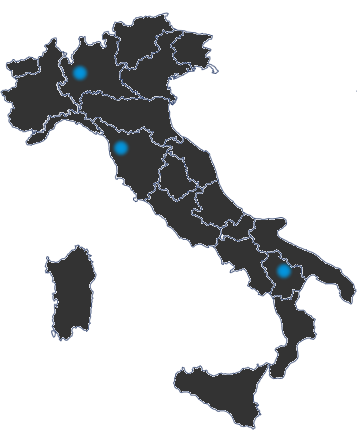
\includegraphics[scale=0.25]{img/italia.png}
    %~
  \section{Languages}
    \textbf{Vietnamese}
\includegraphics[scale=0.40]{img/5stars.png}
    \textbf{English}
\includegraphics[scale=0.40]{img/2stars.png}
    ~
\end{aside}

\section{Volunteer Experience}
Student Volunteer\\
\textbf{Support the activities of the holiday season in Phật Quang Pagoda - Vũng Tàu}\\
\emph{Visit SOS Children's Village (Đông Hòa, Dĩ AN, Bình Dương)}
\\
%\section{Honors \& Awards}
%\begin{entrylist}
  %\entry
  %  {10/2015}
  %  {Best swordsman duel}
  %  {Contest}
  %  {Lorem ipsum.\\
  %  \emph{Lorem ipsum}}
%\end{entrylist}

\section{Certifications}
\begin{entrylist}
  \entry
    {06/2015}
    {TOEIC}
    {IIG Vietnam}
    {\emph{Test of English for International Communication}}
\end{entrylist}

%\section{Other Info}
%For the Italian job market:\\
%\emph{Si autorizza il trattamento delle informazioni contenute nel curriculum in conformità alle disposizioni previste dal %d.lgs. 196/2003. Si dichiara altresì di essere consapevole che, in caso di dichiarazioni non veritiere, si è passibili di sanzioni %penali ai sensi del DPR 445/00 oltre alla revoca dei benefici eventualmente percepiti.}
%\\
\begin{flushleft}
\emph{Jul 17th, 2018}
\end{flushleft}
\begin{flushright}
\emph{Long Nguyen}
\end{flushright}

\end{document}
